\documentclass[english,compress]{beamer}
\usepackage{kloeckislides}
\nonstopmode

\usepackage[normalem]{ulem}
\usepackage{pifont}
\usepackage{ifthen}

\setbeamercolor{section in head/foot}{use=structure,bg=structure.fg!25!bg}
\defbeamertemplate*{footline}{split theme}
{%
  \leavevmode%
  \begin{beamercolorbox}[wd=.5\paperwidth,ht=2.5ex,dp=1.125ex]{section in head/foot}%
    \insertsectionnavigationhorizontal{\paperwidth}{\hskip0pt plus1filll}{}%
  \end{beamercolorbox}%
  %\begin{beamercolorbox}[wd=.5\paperwidth,ht=2.5ex,dp=1.125ex]{subsection in head/foot}%
    %\insertsubsectionnavigationhorizontal{.5\paperwidth}{}{\hskip0pt plus1filll}%
  %\end{beamercolorbox}%
}


%\useoutertheme[subsection=false]{miniframes}

\setbeamertemplate{frametitle}[default][center]

\AtBeginDocument{%
  {
    \usebeamercolor{section in head/foot}
  }
  
  \pgfdeclareverticalshading{beamer@headfade}{\paperwidth}
  {%
    color(0cm)=(bg);
    color(1.25cm)=(section in head/foot.bg)%
  }

  \setbeamercolor{section in head/foot}{bg=}
}

\addtoheadtemplate{\pgfuseshading{beamer@headfade}\vskip-1.25cm}{}

\beamertemplatedotitem

\setbeamercolor{section in head/foot}{parent=palette quaternary}
\setbeamercolor{subsection in head/foot}{parent=palette primary}

\setbeamercolor{author in head/foot}{parent=section in head/foot}
\setbeamercolor{title in head/foot}{parent=subsection in head/foot}



\AtBeginSection[] {
  \begin{frame}<beamer>
  \frametitle{Outline}
  \tableofcontents[sectionstyle=show/shaded,subsectionstyle=show/show/hide]
\end{frame}
}
\AtBeginSubsection[] {
  \begin{frame}<beamer>
  \frametitle{Outline}
  \tableofcontents[sectionstyle=show/shaded,subsectionstyle=show/shaded/hide]
\end{frame}
}

\newcommand{\technicality}[2]{%
  {\strut #1\\
    \begin{beamercolorbox}[sep=1mm]{block body}
      #2
    \end{beamercolorbox}
  }%
}

\lstset{
  language=C++,
  rangebeginprefix=//\ ,
  rangeendprefix=//\ ,
}

\def\weblink#1#2{\href{#1}{\color{blue}\underline{#2}}}

\definecolor{fetch}{RGB}{227,110,35}
\definecolor{alu}{RGB}{255,188,24}
\definecolor{context}{RGB}{132,146,175}

\usepackage{keystroke}

\setbeamertemplate{navigation symbols}{}


\begin{document}
% {{{ front matter

\title{High-Performance Scientific Computing\\Lecture 1: Intro}

\date{MATH-GA 2011 / CSCI-GA 2945 $\cdot$ September 5, 2012}

\frame{\titlepage}

\begin{frame}{Today}
  \tableofcontents[hideallsubsections]
\end{frame}
% }}}
% -----------------------------------------------------------------------------
\section{About this class}
% -----------------------------------------------------------------------------
% {{{
% -----------------------------------------------------------------------------
\begin{frame}{Course Outline}
  \begin{tikzpicture}[overlay]
    \node [above left =1cm of current page.south east,
    rotate=10,opacity=0.3,yshift=1cm] 
    { \includegraphics[width=8cm]{dictionary.jpeg} } ;
  \end{tikzpicture}
  \begin{columns}
    \column{0.5\textwidth}
    \textbf{Part 1: Do} ($\sim 4$)

    \begin{itemize}
      \item Write, run programs (C)
      \item Use tools (make, git, gdb)
      \item OpenMP, MPI, OpenCL
      \item Correctness in each
    \end{itemize}

    \medskip
    \textbf{Part 2: Understand} ($\sim$3)

    \begin{itemize}
      \item Measure and understand performance
      \item Basic machine architecture
      \item CPU machine model
      \item GPU machine model
    \end{itemize}

    \column{0.5\textwidth}
    \textbf{Part 3: Refine} ($\sim$3)

    \begin{itemize}
      \item Advanced tools \& languages
      \item Work partitioning
      \item Common patterns
      \item Load balancing
    \end{itemize}

    \medskip
    \textbf{Part 4: Apply}

    \begin{itemize}
      \item Find a project\\
        (start looking \emph{now}!)
      \item Pitch it to us (5 min)
      \item Apply what you've learned
      \item Present (2)
    \end{itemize}
  \end{columns}
\end{frame}
% -----------------------------------------------------------------------------
\begin{frame}{Grading}
  \Large
  \begin{itemize}
    \item 60\% Weekly homework
    \item 40\% Final project
  \end{itemize}
\end{frame}
% -----------------------------------------------------------------------------
\begin{frame}{Sign-up sheet}
  \begin{center}
    \includegraphics[height=5cm]{notebook.jpeg}
  \end{center}
\end{frame}
\addimgcredit{Notebook: sxc.hu/abeall}
% -----------------------------------------------------------------------------
\begin{frame}{Survey}
  \begin{columns}
    \column{0.5\textwidth}
    \includegraphics[width=\textwidth]{question-mark.jpeg}
    \column{0.5\textwidth}
    \begin{itemize}[<+->]
      \item Home department
      \item Degree
      \item Longest program ever written?
      \item Language?
      \item Parallel?
      \item Already have a project?
    \end{itemize}
  \end{columns}
\end{frame}
\addimgcredit{Question mark: sxc.hu/svilen001}
% -----------------------------------------------------------------------------
\begin{frame}{Listserv}
  \begin{center}
    \Huge
    \href{mailto:hpc12@tiker.net}{hpc12@tiker.net}
  \end{center}
\end{frame}
% -----------------------------------------------------------------------------
\begin{frame}{Smile! You're on camera}
  \begin{center}
    \includegraphics[height=5cm]{camera.jpeg}

    Lecture media will be posted soon after each class.

    (Room audio, lecture audio, screencast, room video)
  \end{center}
\end{frame}
\addimgcredit{Camera: sxc.hu/Kolobsek}
% -----------------------------------------------------------------------------
\begin{frame}{Class web page}
  \begin{center}
    \Huge
    \href{http://bit.ly/hpc12}{bit.ly/hpc12}
  \end{center}
  \uncover<2>{
    \begin{tikzpicture} [overlay]
      \node [above right=1cm of current page.south west,
        draw,drop shadow,fill=white,inner sep=5mm,thick,yshift=2cm]
        {
          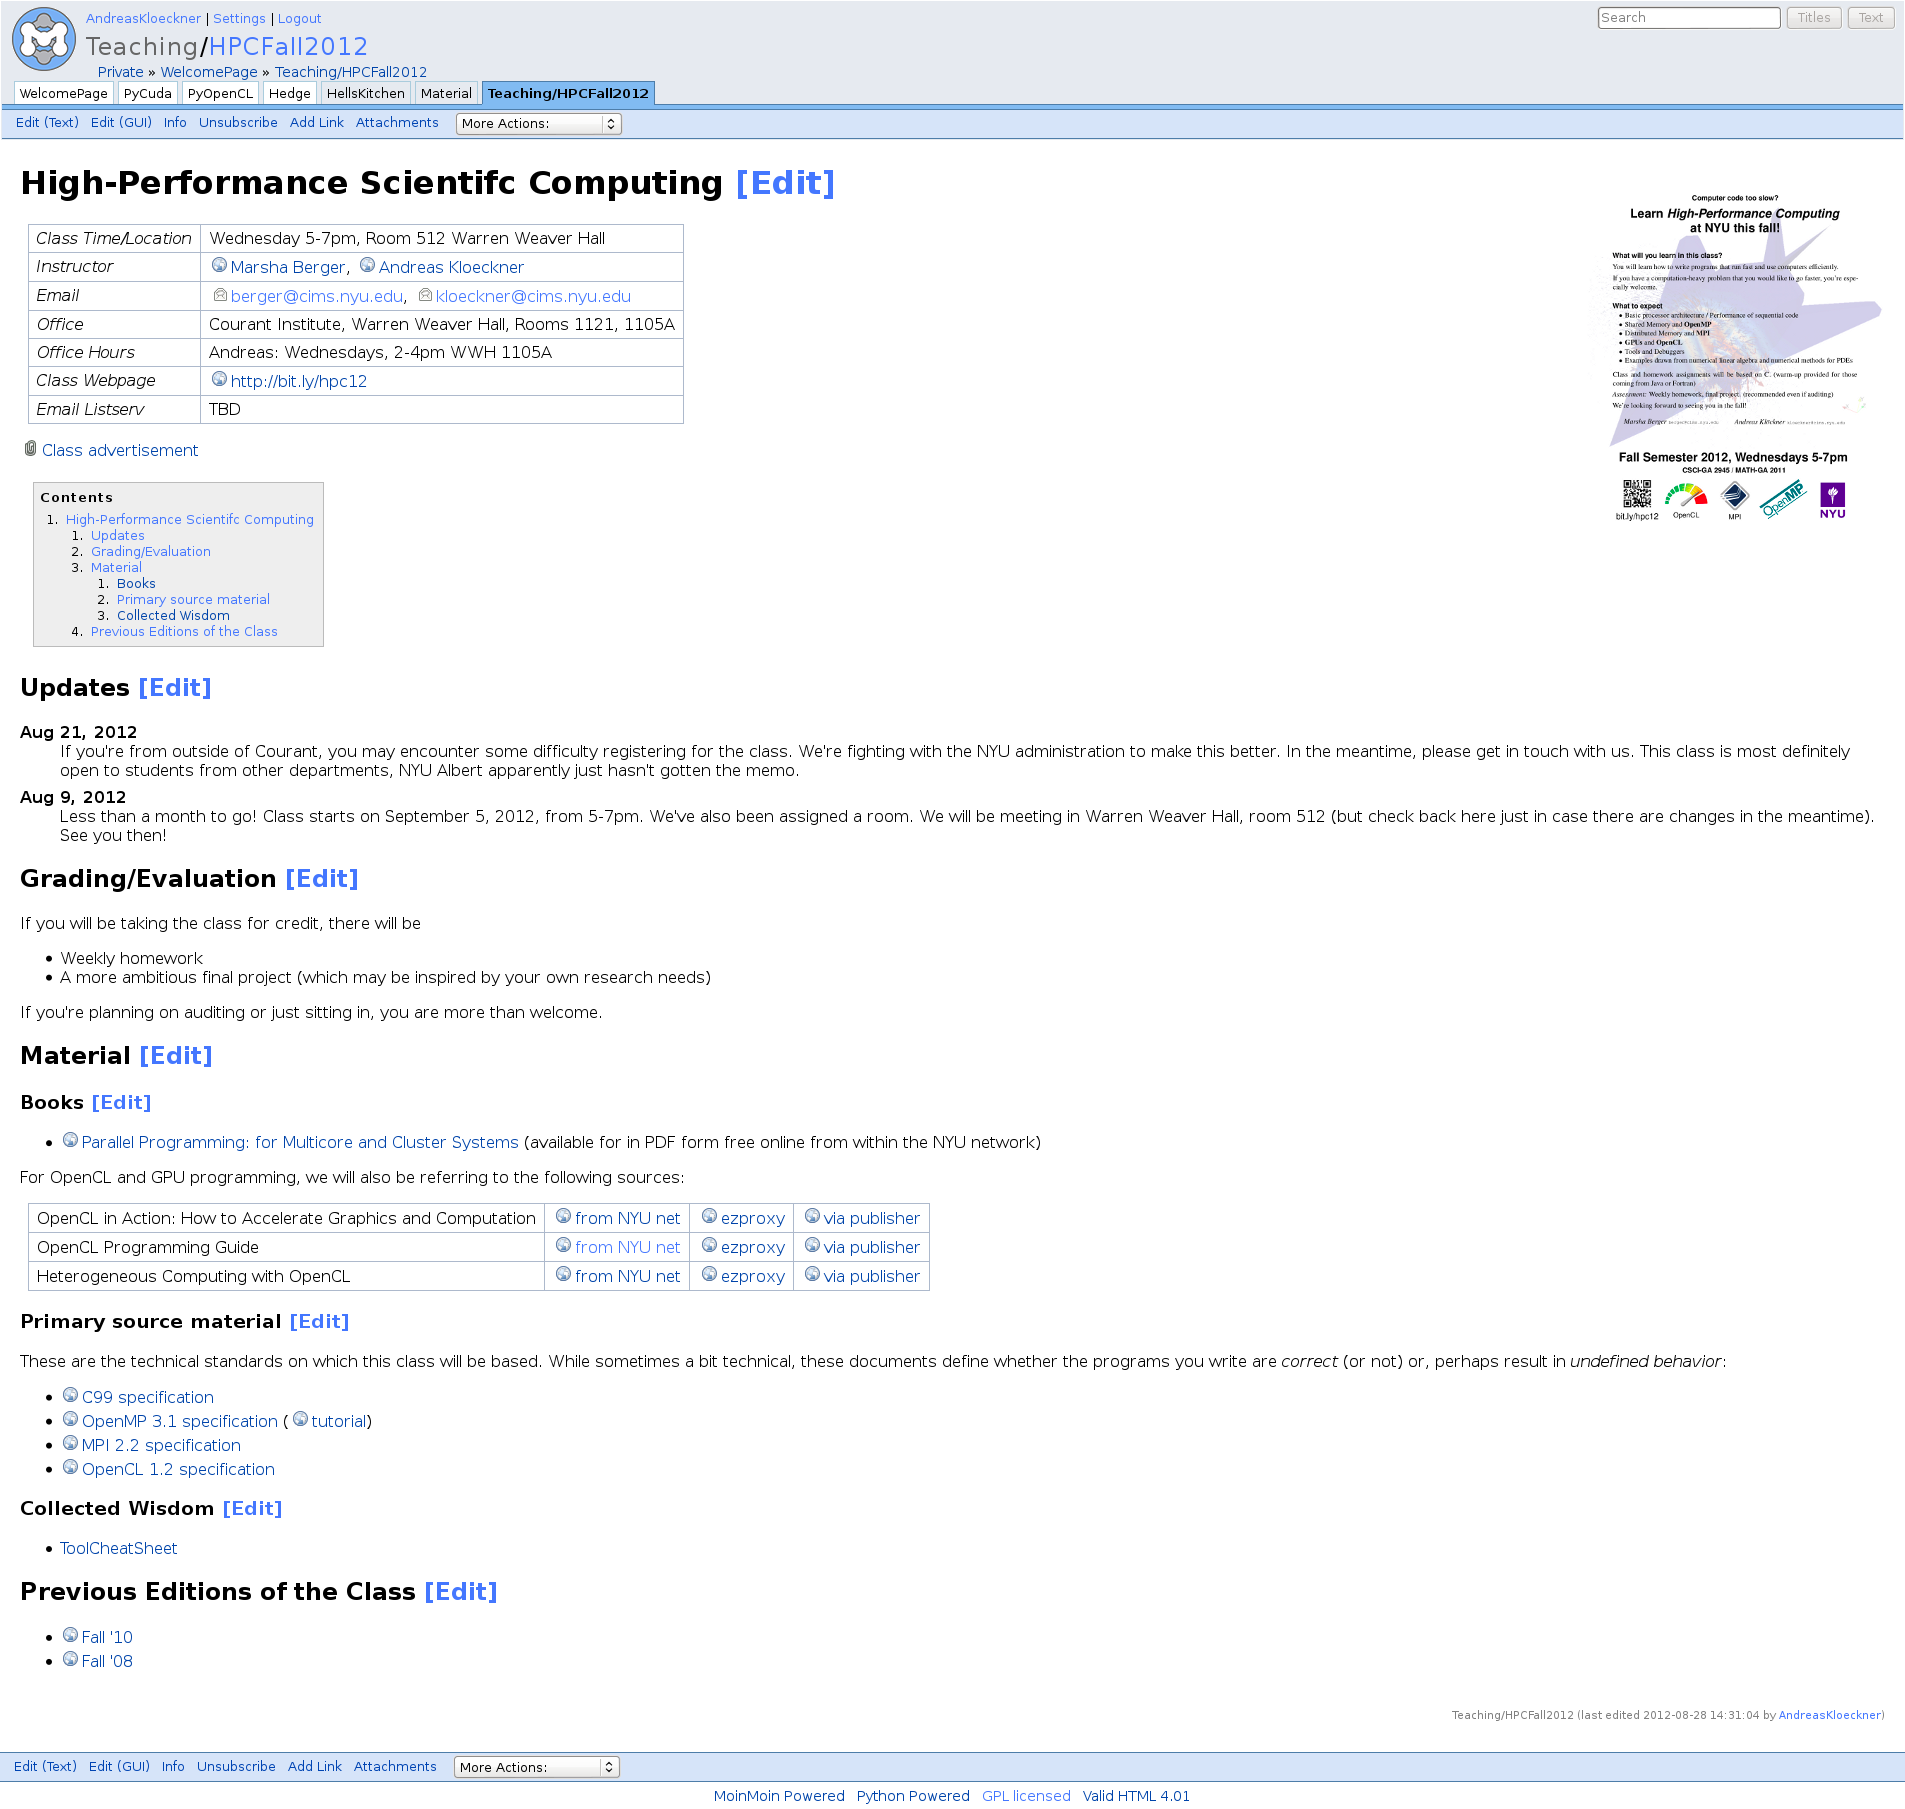
\includegraphics[width=0.5\textwidth]{hpc-web-screenshot.png}
        } ;
    \end{tikzpicture}
  }
  \uncover<2>{
    \begin{tikzpicture} [overlay]
      \node [above left=1cm of current page.south east,
        draw,drop shadow,fill=white,inner sep=5mm,thick,
        text width=0.6\textwidth]
        {
          What's there?
          \begin{itemize}
            \item \emph{Homework 1}, due next week.
            \item 
          \end{itemize}
        } ;
    \end{tikzpicture}
  }
\end{frame}
% }}}
% -----------------------------------------------------------------------------
\section{HPC: A look around}
% -----------------------------------------------------------------------------
% {{{
% }}}
% -----------------------------------------------------------------------------
\section{A taste of what's to come}
% -----------------------------------------------------------------------------
% {{{
% }}}

\questionframe{}
\imagecreditslide

\end{document}
% vim: foldmethod=marker
